%
% Introducción a FPE, presentación de cifrados que preservan el formato.
% Proyecto Lovelace.
%

\subsection{Introducción}

\begin{frame}{Introducción a FPE}
  {Planteamiento del problema}

  Los cifradores estándar (por ejemplo, AES) convierten un mensaje en una
  cadena binaria.

  \begin{figure}[H]
    \begin{center}
      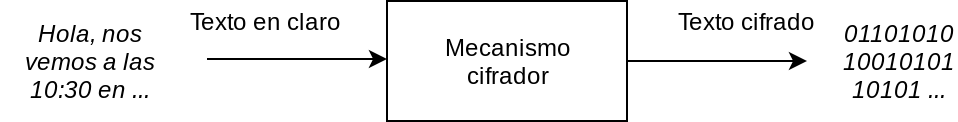
\includegraphics[width=0.75\linewidth]{diagramas/cifrador_estandar.png}
    \end{center}
  \end{figure}

  \onslide<2->

  La cual, al ser interpretada, se compone principalmente de caracteres no
  imprimibles.

  \begin{figure}[H]
    \begin{center}
      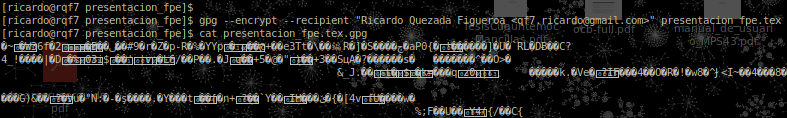
\includegraphics[width=1.0\linewidth]{diagramas/no_imprimibles.png}
    \end{center}
  \end{figure}

  \note<2>
  {
    Generalización de ejemplo a pdf e imágenes: no se espera que un pdf cifrado
    siga siendo un pdf válido; o que una imagen cifrada se siga pudiendo
    ver con un visor de imágenes.
  }

\end{frame}

\begin{frame}{Introducción a FPE}
  {Planteamiento del problema}

  El objeto de los cifrados que preservan el formato
  (\textit{Format-preserving Encryption}, FPE) es convertir un texto en claro
  con un formato dado en un texto cifrado con el mismo formato.

  \begin{figure}[H]
    \begin{center}
      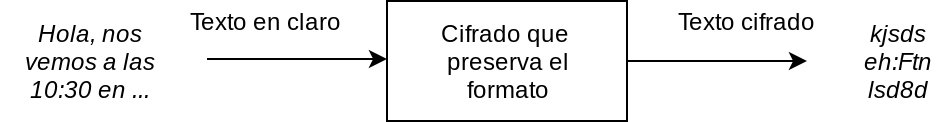
\includegraphics[width=0.75\linewidth]{diagramas/cifrador_formato.png}
    \end{center}
  \end{figure}

  \note<1>
  {
    Para el ejemplo de la figura (un formato de los caracteres ASCII
    imprimibles), no existen muchas aplicaciones reales; es solo con
    fines ilustrativos.
  }

  \onslide<2->

  Formalmente, se busca obtener una permutación

  $$ \mathcal{E}: \mathcal{K} \times \mathcal{X} \rightarrow \mathcal{X} $$

  que sea difícil de invertir sin el conocimiento de la llave.

  \note<2>
  {
    En realidad la ecuación es casi la definición de cifrado común; lo único
    que hay que hacer notar es que \textit{el formato} de $ \mathcal{X} $
    se debe poder reproducir en el texto cifrado.

    También hay que hacer notar cómo, si se ve al formato como una cadena
    binaria, entonces los cifradores estándar son por sí mismos cifrados que
    preservan el formato.
  }

\end{frame}

\begin{frame}{Introducción a FPE}
  {Aplicaciones}

  La utilidad de los cifrados que preservan el formato se centra principalmente
  en \textit{agregar} seguridad a sistemas y protocolos que ya se encuentran
  en un entorno de producción. Estos son algunos ejemplos de dominios
  comunes en FPE:

  \note<1>
  {
    Hablar de en qué contextos se quiere preservar el formato de este tipo
    de datos: bases de datos que los usan como índices, o aplicaciones en
    las que se usan como identificadores.
  }

  \begin{itemize}

    \item<2-> Números de tarjetas de crédito. \\
      \texttt{5827 5423 6584 2154} $ \rightarrow $ \texttt{6512 8417 6398 7423}

    \item<3-> Números de teléfono. \\
      \texttt{55 55 54 75 65} $ \rightarrow $ \texttt{55 55 12 36 98}

    \item<4-> CURP. \\
      \texttt{GHUJ887565HGBTOK01} $ \rightarrow $ \texttt{QRGH874528JUHY01}

  \end{itemize}

  \note<4>
  {
    En algunos casos, se debe mantener cierta parte del texto en claro
    en el texto cifrado (más adelante se hablará de las tarjetas de crédito),
    como en el ejemplo del teléfono.
  }

\end{frame}
